%analysis and solution: mathematics/algorithms/system design

\subsection{System design}

Using wxWidgets we set up a window with the necessary controls to modify parameters with which to generate maps and export them. Within this window we will be using OpenGL to visualize the generation process and provide the user with an idea of what the map might look like in the viewer application.

\subsubsection{Preview rendering}

We want to give the user a good idea of what is being generated and how this is being done. This will highlight the workings of the generation process and allow the user to intuitively judge wether he or she should adjust the parameters.

\paragraph{Shaders}

Whenever we will be rendering anything we will be using appropriate shaders. For now we will be using a pair of relatively simple vertex and fragment shaders to be extended where needed. To start with they take into account the projection, position of the camera and model matrix for whichever object is being drawn. Furthermore each vertex has an associated position, normal and color. These are more or less minimal requirements to render anything. They also consider a single light source to add some dynamics to the map preview. 

Even with these simple shaders we can observe the effect of the calculations of the fragment shader in that eventual lighting dependent output colours are determined not per vertex but per pixel. This is one of the more obvious advantages of using our custom shaders.

\paragraph{Graph visualisation}

To visualize the underlying structure of the maps that we want to generate we needed a method of rendering graphs. Many of the steps in the algorithm rely on modifying attributes of nodes in a graph. For starters we wanted to render the voronoi diagrams which are generated in the first step of the algorithm. Besides giving us an idea of wether they were being generated correctly it resulted in an interesting image which we want te user to be able to access.

%Tim als jij dit ergens anders wil zetten mag dat ik wil er in ieder geval aan refereren
\begin{figure}[h]
	\centering
	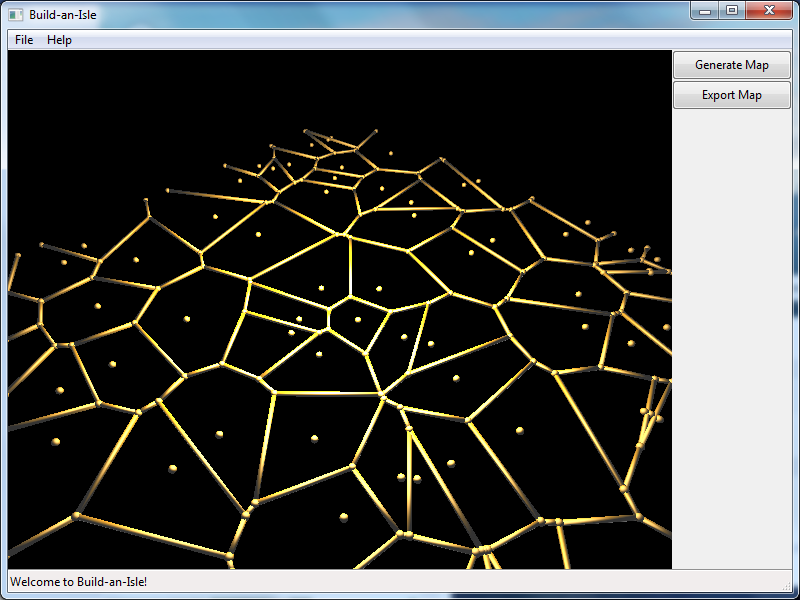
\includegraphics[width=\linewidth]{voronoi-random}
	\caption{Voronoi diagram visualized}
	\label{fig:voronoi-random}
\end{figure}

For each node we render spheres and we use beams to connect them appropriately. By visualizing the graph in 3D we can use the same method in subsequent steps which do make use of the third dimension and have a seamless transition. Figure~\ref{fig:voronoi-random} shows an example of a visualized randomly generated voronoi diagram.